\section{Test}

Un test non può dimostrare la correttezza di un programma, ma può solo dimostrare che è errato.

Perché testare allora?
\begin{itemize}
  \item condfidenza
  \item previene le regressioni, rompiano il codice che prima funzionava
\end{itemize}

inventimento per il futuro. parte essenziale per l'esperizna di èrogrammatore

\paragraph{Esempio}

\begin{minted}[breaklines]{rust}
fn divide(a: i32, b: i32) -> i32 {
  a / b
}
 \end{minted}


ci arrgogiamo che la divisione per zero è gestita in amlo modo solo a runtime.

Ci sono molti tipologie di test. I primi sono l'analisi statica del programma
fronito di default da IDE avanzati come Visual Studio Code o Rustrover

\section{Test di unità}

Un test di unità, o \textbf{unit test}, valuta il comportamento di un singolo componente software
(funzione, struttura dati, …), indipendentemente dal resto del sistema

Piccola funzione che mira ad usare im maniera isolata predicemndole il risultato.
Nel caso di Rust trovmiao la macro assert o notAssert che verifica che l'easpettativa sia
soddisfatta o meno.

Con cargo test vengono esesguite le funzioni di test per verificare se il codice
è sano o meno, anche aggiungendo codice.


I test sollevano un comportamento

\begin{minted}[breaklines]{rust}
#[test]
fn test_divide() {
  assert_eq!(divide(6,3), 2);
}
\end{minted}

\begin{tcolorbox}
  \textbf{Nota:} Verifica un caso tipico ma non copre errori. Un test singolo non
  basta!
\end{tcolorbox}

Proprio per questo motivo dobbiamo andare a testare i casi limite.

Gli unit test sono dei with box text scritti direttamente dal programmatore. Siamo
in grado di predire che determianti parateri in ingresso portano a un certo risultato in uscita.

Eg granello di sabbia in un orologio meccanico vs goccia d'acqua in un orologio al quarzo.

\subsection{Quanti test fare}
La complessità ciclomatica è una misura del numero di for, if etc

Meglio due fuznioi semplici in cascata che una unica.
Spesso si utilizza il refactoring per semplificare il codice.


I test sono importatni averli dall'inizio dopo non hanno senso.

\section{Test dei casi limite}

È fondamentale testare i casi limite. Per questo Rust offre la possibilità
di scrivere \verb|#[should_panic]| avvertendo il compilatore che ci
aspettiamo che la funzione vada in panic.

\begin{minted}[breaklines]{rust}
#[test]
#[should_panic]
fn test_divide_by_zero() {
  divide(10,0);
}
\end{minted}

I test devono verificare:

\begin{itemize}
  \item I casi normali
  \item I casi limite come divisione per 0, accesso al primo e all'ultimo elemento di un contenitore, etc.
  \item La corretta identificazione/gestione/propagazione degli errori
\end{itemize}

\begin{tcolorbox}
  \textbf{Note:} I test servono anche a testare errori!
\end{tcolorbox}

\section{Refactoring: miglioriamo il codice}

Nel momento in cui dobbiamo testare una funzione vi sono due possibilità

I test fanno parte della speficifca del test

\begin{itemize}
  \item Le specifiche specifiche non sono chiare, non sappiamo come gestire un
        errore. I test sono molto utile alla specifica, perché in linguaggio naturale
        sarebbe difficile esprimere tutte le casistiche, altrimenti il lavoro sarebbe
        già fatto
  \item Quando mi rendo conto che il comportamento non può essere determinato
        dal cliente finale dato che è una scelta mia progettuale di cui non è a
        conoscenza il cliente. Non potendomi appelare a lui posso dire che alcune
        volte mi torna un i32 e altre volte nulla o un errore, quindi cambiio la firma usando Option o Result
\end{itemize}

\begin{minted}[breaklines]{rust}
fn divide(a: i32, b: i32) -> Option<i32> {
  if b == 0 { None }
  else { Some(a / b) }
}

#[test]
fn test_divide_safe() {
  assert_eq!(divide(2,1), Some(2));
  assert_eq!(divide(1,0), None);
}
\end{minted}

Questo processo ha reso il nostro codice più safe.

\begin{tcolorbox}
  \textbf{Note:} Niente panic e questo implica un'API più sicura
\end{tcolorbox}

\section{Test di integrazione}

Fino ad ora abbimao visto i singoli test, ma il nostro sistema è un
composto di fuznio che ne chaimano altre e che interagiscono tra loro.

Per questo dobbiamo complicare i test e iniziare a palrale di test di
intrgazione o integration test.

Guardiamo l'interazione tra due o più moduli software per verificare
se funzionano correttamente insieme.

Mentre nell'unit test posso scegliere con presicone i casi limiti in questo caso
li devo trattare a black box. se copllettivamente rispetto all'imput danno
l'output atteso.

Poiché siamo a balckbox applichero l'integratopn test dopo aver testato
i test di unità.

Inoltre gli intregation test sono più difficili e costoso da gestire in caso di errore


\begin{center}
  \begin{minipage}{0.65\linewidth}

  \end{minipage}%
  \hfill
  \begin{minipage}{0.3\linewidth}
    \centering
    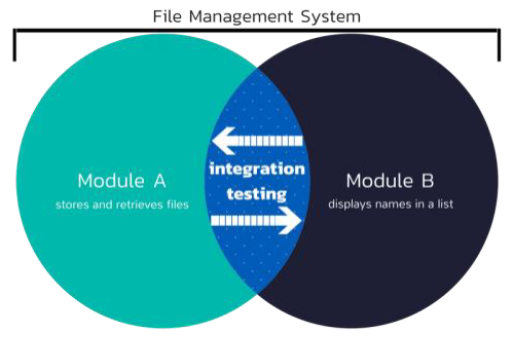
\includegraphics[width=\linewidth]{content/API_Programming/images/2026-03-24-13-43-14.png}
  \end{minipage}
\end{center}


\section{Test di integrazione: modulo Repository}

\begin{minted}[breaklines]{rust}
pub struct OrderRepository {
  data: HashMap<u32, f64>;
}
impl OrderRepository {
  pub fn new() -> Self {
    Self {data: HashMap::new() }
  }
  pub fn save(&mut self, id: u32, v: f64) {
    self.data.insert(id, v);
  }
  pub fn find(&self, id: u32) -> Option<f64>{
    self.data.get(&id).copied()
  }
}
\end{minted}

\begin{center}
  \begin{minipage}{0.65\linewidth}
    Contiene la logica applicativa. Si appoggia sulle funzionalità del
    modulo precedente.
  \end{minipage}%
  \hfill
  \begin{minipage}{0.3\linewidth}
    \begin{minted}[breaklines]{rust}
pub struct OrderService<'a> {
  repo: &'a mut OrderRepository
}
impl<'a> OrderService<'a> {
  pub fn new(repo: &'a mut OrderRepository) -> Self { Self { repo } }
  pub fn apply_discount(&mut self, id: u32) -> Result<f64, String> {
    let t = self.repo.find(id).ok_or("Order not found")?;
    let discounted = if t > 100.0 { t * 0.9 }
                      else { t }
    self.repo.save(id, discounted);
    Ok (discounted)
  }
}
\end{minted}
  \end{minipage}
\end{center}

\subsection{Test di integrazione: esempio di test}

\begin{center}
  \begin{minipage}{0.47\linewidth}
    \begin{minted}[breaklines]{rust}    
// caso normale
#[test]
fn test_apply_discount_integration() {
  // Arrange
  let mut repo = OrderRepository::new();
  repo.save(1, 200.0);
  let mut s = OrderService::new(&mut repo);
  // Act
  let result = s.apply_discount(1);
  // Assert
  assert!(result.is_ok());
  let saved = repo.find(1);
  assert_eq!(saved, Some(180.0));
}
\end{minted}

  \end{minipage}
  \hfill
  \begin{minipage}{0.47\linewidth}
    \begin{minted}[breaklines]{rust}
// caso limite
#[test]
fn test_apply_discount_not_found() {
  // Arrange
  let mut repo = OrderRepository::new();
  let mut s = OrderService::new(&mut repo);
  // Act
  let result = s.apply_discount(42);
  // Assert
  assert!(result.is_err());
}
\end{minted}

  \end{minipage}
\end{center}


\section{Test di integrazione: razionale}

Unit test: verifica una sinola fuznone
Integration test: verifica l'integrazione che il sistema fuznioi


\section{Test complessivi - end-to-end}

Viene fatta solitamente con il cliente e a sistema completo.


\begin{figure}[h!]
	\centering
	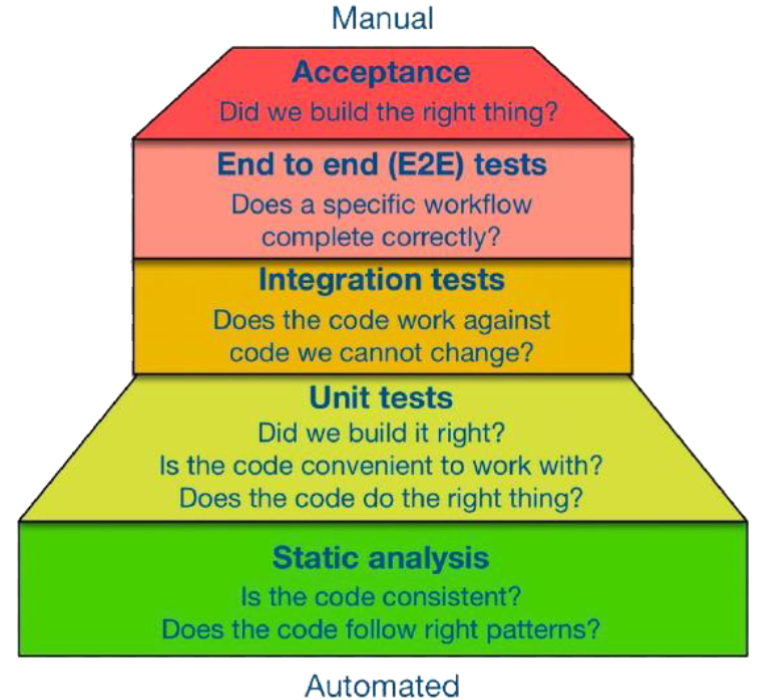
\includegraphics[width=\linewidth]{content/API_Programming/images/2026-03-24-13-59-21.png}
\end{figure}


\section{Cosa fanno i test}

I test trovano i bug ma non possono dimostrale l'assenza di essi.
per poter garantire che non vi sono bug dovremmo avere una logica formale
come per la programazione concorrente.
Eg un mutex può essere usato da uno e un unico thread

I Test forniscono una documentazione del software, miglioranod la compresione
ma anche il design del codice.

\section{Il flusso di lavoro con i test}

\begin{enumerate}
  \item Si scrive una funzione
  \item Si scrivono i test che ne verificano il comportamento
  \item Si esegue cargo test
  \item Si correggono gli errori che vengono riportati
  \item Si ripete fino a che il programma è completo
\end{enumerate}

\section{Test in Rust}

con \verb|#[cfg(test)]| sono con cargo test viene eseguito, altrimenti
il compilatore lo ignora e l'eseguibile è più leggero.


I test di integrazine stanno fuori dal nostro modulo e vedono solo le fuznioni ubliche
Funzionano nìmeglio se abbiamo un main e una lib

\begin{minted}[breaklines]{rust}
// funzione da testare
fn sum(a: i32, b: i32) -> i32 {
  a + b
}

#[cfg(test)]
mod tests {
  fn sum_inputs_outputs() -> Vec<((i32, i32), i32)> {
    vec![((1, 1), 2), ((0, 0), 0), ((2, -2), 0)]
  }
  #[test]
  fn test_sums() {
    for (input, output) in sum_inputs_outputs() {
     assert_eq!(crate::sum(input.0, input.1), output);
    }
  }
}
\end{minted}


\section{Sintassi dei test}

Vi è una sintassi chiamata \textbf{AAA}:

\begin{itemize}
  \item Arrange: Preparazione dei valori su cui operare
  \item Act: Esecuzione del codice da testare
  \item Assert: Verifica, mediante asserzioni, che i risultati ottenuti siano
\end{itemize}


\begin{center}
  \begin{minipage}{0.65\linewidth}
    
  \end{minipage}%
  \hfill
  \begin{minipage}{0.3\linewidth}
    \begin{minted}[breaklines]{rust}
#[test]
fn test_divide_aaa() {
// Arrange
let a = 6;
let b = 2;
// Act
let result = divide(a, b);
// Assert
assert_eq!(result, 3);
}
\end{minted}
  \end{minipage}
\end{center}

perché usare assert\_eq rispetto che assert? 
quando eq si rompe, eq(5, 7), mi aspettavo 7 mi hai dato 5.


\section{Eseguire i test}

Usando \verb|cargo test| vengono invocate tutte le funzioni di test.
prima unit poi integration naviganndo tra le varie cartelle del progetto.


Quando la base di test è molto almpia pure i tempo auemnta. usiamo 

--ignored 

\section{Automatizzare la creazione di test}
Alcui sistemi devono essere provati con molti dati diversi, una lib può essere
rstest dando la possibilità di scrivere funzioni con parametri paramtrici
invocando la funzione test più volte tante quante sono i case definiti.



\begin{minted}[breaklines]{rust}
use rstest::rstest;
#[rstest]
#[case(1, 2, 3)]
#[case(0, 0, 0)]
#[case(-1, 1, 0)]
fn test_sum(#[case] a: i32,
            #[case] b: i32,
            #[case] expected: i32) {
  assert_eq!(sum(a, b), expected);
}
\end{minted}











